\documentclass{beamer}\usepackage[]{graphicx}\usepackage[]{color}
%% maxwidth is the original width if it is less than linewidth
%% otherwise use linewidth (to make sure the graphics do not exceed the margin)
\makeatletter
\def\maxwidth{ %
  \ifdim\Gin@nat@width>\linewidth
    \linewidth
  \else
    \Gin@nat@width
  \fi
}
\makeatother

\definecolor{fgcolor}{rgb}{1, 0.894, 0.769}
\newcommand{\hlnum}[1]{\textcolor[rgb]{0.824,0.412,0.118}{#1}}%
\newcommand{\hlstr}[1]{\textcolor[rgb]{1,0.894,0.71}{#1}}%
\newcommand{\hlcom}[1]{\textcolor[rgb]{0.824,0.706,0.549}{#1}}%
\newcommand{\hlopt}[1]{\textcolor[rgb]{1,0.894,0.769}{#1}}%
\newcommand{\hlstd}[1]{\textcolor[rgb]{1,0.894,0.769}{#1}}%
\newcommand{\hlkwa}[1]{\textcolor[rgb]{0.941,0.902,0.549}{#1}}%
\newcommand{\hlkwb}[1]{\textcolor[rgb]{0.804,0.776,0.451}{#1}}%
\newcommand{\hlkwc}[1]{\textcolor[rgb]{0.78,0.941,0.545}{#1}}%
\newcommand{\hlkwd}[1]{\textcolor[rgb]{1,0.78,0.769}{#1}}%
\let\hlipl\hlkwb

\usepackage{framed}
\makeatletter
\newenvironment{kframe}{%
 \def\at@end@of@kframe{}%
 \ifinner\ifhmode%
  \def\at@end@of@kframe{\end{minipage}}%
  \begin{minipage}{\columnwidth}%
 \fi\fi%
 \def\FrameCommand##1{\hskip\@totalleftmargin \hskip-\fboxsep
 \colorbox{shadecolor}{##1}\hskip-\fboxsep
     % There is no \\@totalrightmargin, so:
     \hskip-\linewidth \hskip-\@totalleftmargin \hskip\columnwidth}%
 \MakeFramed {\advance\hsize-\width
   \@totalleftmargin\z@ \linewidth\hsize
   \@setminipage}}%
 {\par\unskip\endMakeFramed%
 \at@end@of@kframe}
\makeatother

\definecolor{shadecolor}{rgb}{.97, .97, .97}
\definecolor{messagecolor}{rgb}{0, 0, 0}
\definecolor{warningcolor}{rgb}{1, 0, 1}
\definecolor{errorcolor}{rgb}{1, 0, 0}
\newenvironment{knitrout}{}{} % an empty environment to be redefined in TeX

\usepackage{alltt}
\usepackage{../371g-slides}
\usepackage{preview}
\title{Dummy Variables}
\subtitle{Lecture 14}
\author{STA 371G}
\IfFileExists{upquote.sty}{\usepackage{upquote}}{}
\begin{document}
  
  
  

  \frame{\maketitle}

  % Show outline at beginning of each section
  \AtBeginSection[]{ 
    \begin{frame}<beamer>
      \tableofcontents[currentsection]
    \end{frame}
  }

  %%%%%%% Slides start here %%%%%%%

  \begin{darkframes}
    \begin{frame}
      \fontsize{9}{9}\selectfont
      Let's predict fuel economy (miles per gallon) for different car models of the 70s.
      
      \begin{center}
        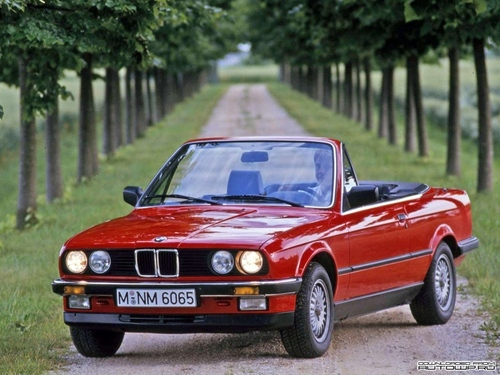
\includegraphics[width=2.8in]{bmw} \\
      \end{center} \pause
      
      \begin{columns}[onlytextwidth]
        \column{.5\textwidth}
          \begin{itemize}
            \item Cylinders
            \item Displacement
            \item Horsepower
          \end{itemize}
        \column{.5\textwidth}
          \begin{itemize}
            \item Weight
            \item Acceleration
            \item Year (After 1975 or not)
          \end{itemize}
      \end{columns}
    \end{frame}
    
    
\begin{frame}[fragile]{Exploring the data}
      \fontsize{9}{9}\selectfont
      Let's display the first 5 rows (and all columns).
\begin{knitrout}
\definecolor{shadecolor}{rgb}{0.137, 0.137, 0.137}\begin{kframe}
\begin{alltt}
\hlstd{auto_mpg[}\hlnum{1}\hlopt{:}\hlnum{5}\hlstd{,]}
\end{alltt}
\begin{verbatim}
# A tibble: 5 x 7
    MPG Cylinders Displacement    HP Weight Acceleration After1975
  <dbl>     <int>        <dbl> <int>  <int>        <dbl>     <chr>
1    18         8          307   130   3504           12        No
2    15         8          350   165   3693           12        No
3    18         8          318   150   3436           11        No
4    16         8          304   150   3433           12        No
5    17         8          302   140   3449           10        No
\end{verbatim}
\end{kframe}
\end{knitrout}
      \pause
      How do we handle the Yes/No data in the ``After1975'' column?
\end{frame}
    
    
    
    
\begin{frame}[fragile]%{Exploring the data}
      \note{This slide is to get familiar with boxplots. Conclusion: Being manufactured after 1975 matters}
\begin{knitrout}
\definecolor{shadecolor}{rgb}{0.137, 0.137, 0.137}\begin{kframe}
\begin{alltt}
\hlkwd{boxplot}\hlstd{(MPG} \hlopt{~} \hlstd{After1975,} \hlkwc{data}\hlstd{=auto_mpg,} \hlkwc{ylab}\hlstd{=}\hlstr{"MPG"}\hlstd{,}
              \hlkwc{xlab}\hlstd{=}\hlstr{"After 1975"}\hlstd{,} \hlkwc{col}\hlstd{=}\hlstr{'darkgray'}\hlstd{)}
\end{alltt}
\end{kframe}
\input{/tmp/figures/unnamed-chunk-4-1.tikz}

\end{knitrout}
      
\end{frame}
    
    
    
\begin{frame}[fragile]{Exploring the data}
        To incorporate the ``After1975'' variable into a regression model, 
        create a \alert{dummy variable} that maps a ``Yes'' to 1, and ``No'' to 0. \pause
\begin{knitrout}
\definecolor{shadecolor}{rgb}{0.137, 0.137, 0.137}\begin{kframe}
\begin{alltt}
\hlstd{auto_mpg}\hlopt{$}\hlstd{LateModel} \hlkwb{<-}
  \hlkwd{ifelse}\hlstd{(auto_mpg}\hlopt{$}\hlstd{After1975} \hlopt{==} \hlstr{"Yes"}\hlstd{,} \hlnum{1}\hlstd{,} \hlnum{0}\hlstd{)}
\end{alltt}
\end{kframe}
\end{knitrout}
      \pause  
      Now let's a regression model using the predictors Cylinders, Displacement, HP, Weight, Acceleration and LateModel.
    
      \lc
\end{frame}
    
    
    
    
\begin{frame}[fragile]{Regression with categorical variables}
      R will actually create this ``dummy'' (0/1) variable for us automatically! \pause
\begin{knitrout}
\definecolor{shadecolor}{rgb}{0.137, 0.137, 0.137}\begin{kframe}
\begin{alltt}
\hlstd{model} \hlkwb{<-} \hlkwd{lm}\hlstd{(MPG} \hlopt{~} \hlstd{Cylinders} \hlopt{+} \hlstd{Displacement} \hlopt{+} \hlstd{HP}
            \hlopt{+} \hlstd{Weight} \hlopt{+} \hlstd{Acceleration} \hlopt{+} \hlstd{After1975,}
            \hlkwc{data}\hlstd{=auto_mpg)}
\hlkwd{summary}\hlstd{(model)}\hlopt{$}\hlstd{r.squared}
\end{alltt}
\begin{verbatim}
[1] 0.78
\end{verbatim}
\end{kframe}
\end{knitrout}
      \pause
      
      R was able to handle the ``After1975'' column, which is a \alert{categorical variable} (or a \alert{factor} as R calls them).
\end{frame}
    
    
    
    
\begin{frame}[fragile]{Dummy variables}
\begin{knitrout}
\definecolor{shadecolor}{rgb}{0.137, 0.137, 0.137}\begin{kframe}
\begin{alltt}
\hlkwd{round}\hlstd{(}\hlkwd{summary}\hlstd{(model)}\hlopt{$}\hlstd{coefficients,} \hlnum{2}\hlstd{)}
\end{alltt}
\begin{verbatim}
             Estimate Std. Error t value Pr(>|t|)
(Intercept)     42.19       2.37   17.81     0.00
Cylinders       -0.58       0.36   -1.62     0.11
Displacement     0.01       0.01    0.94     0.35
HP              -0.02       0.01   -1.35     0.18
Weight          -0.01       0.00   -8.33     0.00
Acceleration     0.04       0.11    0.32     0.75
After1975Yes     4.36       0.40   10.85     0.00
\end{verbatim}
\end{kframe}
\end{knitrout}
      R has created a \alert{dummy variable} ``After1975Yes.''
\end{frame}
    
    
    
\begin{frame}[fragile]{Dummy variables}
      ``After1975Yes'' is 1 whenever ``After1975'' is ``Yes,'' and 0 otherwise:
    
      \begin{table}[!b]
        {\carlitoTLF % Use monospaced lining figures
        \begin{tabularx}{\textwidth}{rrrrr}
           
           MPG &  ... & Acceleration & After1975 & After1975Yes\\ 
          \toprule
            ... & ... & ... & ... & ... \\
            25 & ... & 13.5 & No & 0 \\
            33 & ... & 17.5 & No & 0 \\
            28 & ... & 15.5 & Yes & 1 \\
            25 & ... & 16.9 & Yes & 1 \\
            ... & ... & ... & ... & ... \\
          \bottomrule
            
        \end{tabularx}}
        
      \end{table} 
      
      \pause
      Notice that we do not have a ``After1975No'' variable.\pause
      
      It would cause problems because it would be perfectly correlated with ``After1975Yes.''
\end{frame}
      
      
\begin{frame}[fragile]{Regression with categorical variables}
        Let's simplify our model by omitting statistically insignificant variables one by one. (Make sure to re-run the model after omitting each variable, starting with the least signfiicant.)
        
        What is the $R^2$ in your final model?
        \lc
      
\end{frame}
      
      
      
\begin{frame}[fragile]{Regression with categorical variables}
        \fontsize{9}{9}\selectfont
\begin{knitrout}
\definecolor{shadecolor}{rgb}{0.137, 0.137, 0.137}\begin{kframe}
\begin{alltt}
\hlstd{model} \hlkwb{<-} \hlkwd{lm}\hlstd{(MPG} \hlopt{~}  \hlstd{HP} \hlopt{+} \hlstd{Weight} \hlopt{+} \hlstd{After1975,}
                   \hlkwc{data}\hlstd{=auto_mpg)}
\hlkwd{summary}\hlstd{(model)}\hlopt{$}\hlstd{r.squared}
\end{alltt}
\begin{verbatim}
[1] 0.77
\end{verbatim}
\begin{alltt}
\hlkwd{round}\hlstd{(}\hlkwd{summary}\hlstd{(model)}\hlopt{$}\hlstd{coefficients,} \hlnum{2}\hlstd{)}
\end{alltt}
\begin{verbatim}
             Estimate Std. Error t value Pr(>|t|)
(Intercept)     41.71       0.78    53.1     0.00
HP              -0.02       0.01    -2.3     0.02
Weight          -0.01       0.00   -13.8     0.00
After1975Yes     4.33       0.40    10.8     0.00
\end{verbatim}
\end{kframe}
\end{knitrout}
        \pause
        Is Horsepower capturing the information in Cylinders, Displacement and Acceleration?
      
\end{frame}
      
      
      
\begin{frame}[fragile]{Regression with categorical variables}
        Let's look at the correlations between variables:
        
        {
          \fontsize{9}{9}\selectfont
\begin{knitrout}
\definecolor{shadecolor}{rgb}{0.137, 0.137, 0.137}\begin{kframe}
\begin{alltt}
\hlkwd{cor}\hlstd{(auto_mpg[,}\hlkwd{c}\hlstd{(}\hlnum{1}\hlstd{,}\hlnum{2}\hlstd{,}\hlnum{3}\hlstd{,}\hlnum{4}\hlstd{,}\hlnum{5}\hlstd{,}\hlnum{6}\hlstd{)])}
\end{alltt}
\begin{verbatim}
               MPG Cylinders Displacement    HP Weight Acceleration
MPG           1.00     -0.78        -0.81 -0.78  -0.83         0.42
Cylinders    -0.78      1.00         0.95  0.84   0.90        -0.50
Displacement -0.81      0.95         1.00  0.90   0.93        -0.54
HP           -0.78      0.84         0.90  1.00   0.86        -0.69
Weight       -0.83      0.90         0.93  0.86   1.00        -0.42
Acceleration  0.42     -0.50        -0.54 -0.69  -0.42         1.00
\end{verbatim}
\end{kframe}
\end{knitrout}
        }
        We have \alert{multicollinearity} between HP, Cylinders, Displacement, and Acceleration --- all are highly correlated so it only makes sense to have one of these in the model.
\end{frame}
      
      
      
\begin{frame}[fragile]{Regression with categorical variables}
        The information in Displacement is already mostly captured by HP:
\begin{knitrout}
\definecolor{shadecolor}{rgb}{0.137, 0.137, 0.137}\begin{kframe}
\begin{alltt}
\hlkwd{plot}\hlstd{(auto_mpg}\hlopt{$}\hlstd{HP, auto_mpg}\hlopt{$}\hlstd{Displacement,} \hlkwc{pch}\hlstd{=}\hlnum{16}\hlstd{,}
  \hlkwc{xlab}\hlstd{=}\hlstr{'HP'}\hlstd{,} \hlkwc{ylab}\hlstd{=}\hlstr{'Displacement'}\hlstd{,}\hlkwc{col}\hlstd{=}\hlstr{'green'}\hlstd{,} \hlkwc{main}\hlstd{=}\hlstr{''}\hlstd{)}
\end{alltt}
\end{kframe}
\input{/tmp/figures/unnamed-chunk-11-1.tikz}

\end{knitrout}
\end{frame}
      
      
      
\begin{frame}[fragile]{Interpretation of the $\hat\beta$ of the dummy variable}
        Our regression equation is:
        \[
          \widehat{\text{MPG}} = 41.71 -
          0.02 \cdot \text{HP} -
          0.01 \cdot \text{Weight} +
          4.33 \cdot \text{After1975Yes}.
        \] 
        \pause

        Let's interpret the coefficient 4.33.
        Consider this:
        \begin{itemize}[<+->]
          \item Model A and B have the same HP and Weight.
          \item Model A was manufactured before 1975, whereas B was manufactured after 1975.
          \item We predict Model B will have a MPG that is 4.33 higher than Model A.
        \end{itemize} 
        \lc
\end{frame}
      
      
      
      
\begin{frame}[fragile]{Interpretation of the $\hat\beta$ of the dummy variable}
        R has assigned ``Yes'' to 1 and ``No'' to 0 in our dummy variable, so the ``reference level'' is cars manufactured before 1975.
        \pause\bigskip
	
        If we created a dummy variable After1975No that is 1 for cars manufactured \emph{before} 1975, what would the regression look like?          
\end{frame}
      
      
      
      
      
      
      
\begin{frame}[fragile]{What if there are more than two categories?}
        The Origin variable represents the country of manufacture.
        \fontsize{8}{8}\selectfont
\begin{knitrout}
\definecolor{shadecolor}{rgb}{0.137, 0.137, 0.137}\begin{kframe}
\begin{alltt}
\hlstd{auto_mpg_all[}\hlnum{1}\hlopt{:}\hlnum{5}\hlstd{,]}
\end{alltt}
\begin{verbatim}
# A tibble: 5 x 8
    MPG Cylinders Displacement    HP Weight Acceleration After1975 Origin
  <dbl>     <int>        <dbl> <int>  <int>        <dbl>     <chr>  <chr>
1    18         8          307   130   3504           12        No     US
2    15         8          350   165   3693           12        No     US
3    18         8          318   150   3436           11        No     US
4    16         8          304   150   3433           12        No     US
5    17         8          302   140   3449           10        No     US
\end{verbatim}
\begin{alltt}
\hlkwd{levels}\hlstd{(}\hlkwd{as.factor}\hlstd{(auto_mpg_all}\hlopt{$}\hlstd{Origin))}
\end{alltt}
\begin{verbatim}
[1] "EU" "JP" "US"
\end{verbatim}
\end{kframe}
\end{knitrout}
\end{frame}
      
\begin{frame}[fragile]%{Exploring the data}
        \fontsize{9}{9}\selectfont
\begin{knitrout}
\definecolor{shadecolor}{rgb}{0.137, 0.137, 0.137}\begin{kframe}
\begin{alltt}
\hlkwd{boxplot}\hlstd{(MPG} \hlopt{~} \hlstd{Origin,} \hlkwc{data}\hlstd{=auto_mpg_all,} \hlkwc{ylab}\hlstd{=}\hlstr{"MPG"}\hlstd{,}
              \hlkwc{xlab}\hlstd{=}\hlstr{"Origin"}\hlstd{,} \hlkwc{col}\hlstd{=}\hlstr{'darkgray'}\hlstd{)}
\end{alltt}
\end{kframe}
\input{/tmp/figures/unnamed-chunk-13-1.tikz}

\end{knitrout}
      
\end{frame}
      
      
      
\begin{frame}[fragile]{Regression with categorical variables}
        \fontsize{9}{9}\selectfont
\begin{knitrout}
\definecolor{shadecolor}{rgb}{0.137, 0.137, 0.137}\begin{kframe}
\begin{alltt}
\hlstd{omodel} \hlkwb{<-} \hlkwd{lm}\hlstd{(MPG} \hlopt{~} \hlstd{HP} \hlopt{+} \hlstd{Weight} \hlopt{+} \hlstd{After1975} \hlopt{+} \hlstd{Origin,}
            \hlkwc{data}\hlstd{=auto_mpg_all)}
\hlkwd{round}\hlstd{(}\hlkwd{summary}\hlstd{(omodel)}\hlopt{$}\hlstd{coefficients,}\hlnum{3}\hlstd{)}
\end{alltt}
\begin{verbatim}
             Estimate Std. Error t value Pr(>|t|)
(Intercept)    40.182       0.87    46.0    0.000
HP             -0.028       0.01    -2.8    0.005
Weight         -0.005       0.00   -10.8    0.000
After1975Yes    4.334       0.39    11.0    0.000
OriginJP        1.001       0.61     1.6    0.103
OriginUS       -1.593       0.56    -2.8    0.005
\end{verbatim}
\end{kframe}
\end{knitrout}
        \pause
        \fontsize{10}{10}\selectfont
        For Origin, R has chosen EU as the reference level and create dummy variables for both JP and US.
\end{frame}
      
      

      
\begin{frame}[fragile]{A warning about categorical variables with numeric representations}
        \fontsize{9}{9}\selectfont
          In the original dataset, the origin was represented as 1 for U.S., 2 for EU and 3 for JP.
          \bigskip  \pause
	  
          We would NOT want to just put these numbers in the regression as numbers, because then regression would treat this as if it were a quantitative variable!        
          \bigskip  \pause
	  
          Even though the representation in the file is numeric, it is still a categorical variable and should be treated as such.
      
\end{frame}
      
      
      
\begin{frame}[fragile]{Assumptions}
        \fontsize{9}{9}\selectfont
        What are the issues with this model?
        \lc
\begin{knitrout}
\definecolor{shadecolor}{rgb}{0.137, 0.137, 0.137}\begin{kframe}
\begin{alltt}
\hlkwd{plot}\hlstd{(}\hlkwd{predict.lm}\hlstd{(omodel),} \hlkwd{resid}\hlstd{(omodel),} \hlkwc{col}\hlstd{=}\hlstr{'green'}\hlstd{,} \hlkwc{main}\hlstd{=}\hlstr{''}\hlstd{)}
\end{alltt}
\end{kframe}
\input{/tmp/figures/unnamed-chunk-15-1.tikz}

\end{knitrout}
      
\end{frame}
      
      
      
\begin{frame}[fragile]{Assumptions}
      \fontsize{9}{9}\selectfont
        What about normality?
\begin{knitrout}
\definecolor{shadecolor}{rgb}{0.137, 0.137, 0.137}\begin{kframe}
\begin{alltt}
  \hlkwd{hist}\hlstd{(}\hlkwd{resid}\hlstd{(omodel),} \hlkwc{col}\hlstd{=}\hlstr{'green'}\hlstd{,} \hlkwc{main}\hlstd{=}\hlstr{''}\hlstd{)}
\end{alltt}
\end{kframe}
\input{/tmp/figures/unnamed-chunk-16-1.tikz}

\end{knitrout}
      
\end{frame}
      
      
\begin{frame}[fragile]{Assumptions}
        \fontsize{9}{9}\selectfont
        What about normality?
        
\begin{knitrout}
\definecolor{shadecolor}{rgb}{0.137, 0.137, 0.137}\begin{kframe}
\begin{alltt}
  \hlkwd{qqnorm}\hlstd{(}\hlkwd{resid}\hlstd{(omodel),} \hlkwc{col}\hlstd{=}\hlstr{'green'}\hlstd{,} \hlkwc{main}\hlstd{=}\hlstr{''}\hlstd{)}
\end{alltt}
\end{kframe}
\input{/tmp/figures/unnamed-chunk-17-1.tikz}

\end{knitrout}
      
\end{frame}

\begin{frame}[fragile]{Statistical significance of a categorical variable}
        While dealing with categorical variables, we want to look at the significance of the categorical variable as a whole, rather than looking at $p$-values of individual dummy variables.

        \bigskip\pause

        We want to test the \alert{compound null hypothesis} 
        \[
          H_0 : \beta_{\text{US}} = \beta_{\text{JP}} = 0.
        \]
\end{frame}
      
\begin{frame}[fragile]{Statistical significance of a categorical variable}
        To do this, we look at the ANOVA table; the $p$-value on the Origin line ($2.4 \times 10^{-5}$) is the $p$-value for the compound null hypothesis $H_0 : \beta_{\text{US}} = \beta_{\text{JP}} = 0$.
        \fontsize{9}{9}\selectfont
\begin{knitrout}
\definecolor{shadecolor}{rgb}{0.137, 0.137, 0.137}\begin{kframe}
\begin{alltt}
\hlkwd{anova}\hlstd{(omodel)}
\end{alltt}
\begin{verbatim}
Analysis of Variance Table

Response: MPG
           Df Sum Sq Mean Sq F value  Pr(>F)    
HP          1  14433   14433  1096.0 < 2e-16 ***
Weight      1   2392    2392   181.6 < 2e-16 ***
After1975   1   1623    1623   123.2 < 2e-16 ***
Origin      2    288     144    10.9 2.4e-05 ***
Residuals 386   5083      13                    
---
Signif. codes:  0 '***' 0.001 '**' 0.01 '*' 0.05 '.' 0.1 ' ' 1
\end{verbatim}
\end{kframe}
\end{knitrout}
\end{frame}
      
\begin{frame}{Practical significance of a categorical variable}
        Since $p<.05$, we can conclude that Origin is a statistically significant predictor of MPG.
        But is it a \emph{practically} significant predictor?
        
        \bigskip\pause
        
        To do this, compare $R^2$ values, or standard error of residuals:

        \bigskip

        \begin{tabular}{lll}
        \textbf{Model} & \textbf{$R^2$} & \textbf{Residual standard error} \\
        \hline
        Without Origin in model & 0.77 & 3.72 \\
        With Origin in model & 0.79 & 3.63 \\
        \hline
        \end{tabular}

        \bigskip

        We have to decide if the increased precision is worth the extra complexity in the model.
\end{frame}
 
  \end{darkframes}

\end{document}
